\chapter{La Composition des services web}
%% TODO Introduire la notion de la composition et le plan du chapitre

%   % Dans le chapitres précédent, nous avons étudiés la description, la
% publication,  la découverte et la sélection de services Web
% élémentaire. L'autre concept fondamentale % est la composition des
% services web.


  
%   % The other fundamental concept is web service composition which
% sometimes overlaps or will merge with the process of WS
% discovery. WS composition is a mechanism of combining two or more
% basic services into a possibly complex service. It is used to solve
% complex problems by combining available basic services. It helps to
% accelerate rapid application development and facilitate service
% reuse from developer perspective % and from user perspective it
% increases complex service consumption. As mentioned earlier a
% composite service can be regarded as a combination of services invoked
% in % a predefined order and executed as a whole and that has more
% functionality than its components. WS composition is needed because
% finding a right service provider for the request is not an easy task
% on fast growing WWW sometimes it is even % impossible. Thus WS
% composition becomes necessary and inevitable. Composing WS from
% existing ones is an effective method to fill this gap.\cite{Omer2011}

%   Dans ce chapitre, nous présentons dans un premier temps les
% définitions et les types de composition de services Web présents dans
% la littérature. Ensuite, nous étudions .....
%   Enfin, un ensemble de travaux proposent des approches de la
% composition dynamiques des services web sémantiques.
  

\newpage

  \section{Définition et stratégies de composition}
  \label{sec:defin-et-caract}

  Cette section a pour but d'exposer, d'une part, quelques définitions
  et objectifs de la composition des services Web proposées par la
  communauté, et d'autre part, les différents types et mécanismes de
  composition selon différents points de vue rencontrés dans la
  littérature.
  
    \subsection{Définitions}
    \label{sec:definitions}

    Martin \emph{et al.} \cite{martin2004owl} définissent
    la composition comme étant \emph{``le processus de sélection, de
      combinaison et d'exécution de services en vue
      d'accomplir un objectif donné''}.\\
    % TODO discussion de la définition.

    Selon S. Dustdar et W. Schreiner \cite{dustdar2005survey} :
    \emph{`` L'infrastructure de base des services Web suffit pour la
      mise en œuvre d'interactions simples entre un client et un
      service Web. Si la mise en œuvre d'une application métier
      implique l'invocation d'autres services web, il est nécessaire
      donc de combiner les fonctionnalités de plusieurs services
      web. Dans ce cas, nous parlons d'une composition de services
      Web''}.\\

    % TODO discussion.
    En d'autre terme, La composition de services Web désigne une
    opération qui consiste à construire de nouvelles applications ou
    services appelés \textbf{services composites} ou agrégats par
    l'assemblage ou l'agrégation de services existants nommés
    \textbf{services atomiques} ou élémentaires.

    % TODO: A composite service is defined as a conglomeration of outsourced
    % Web services (called participant services) working in tandem to
    % offer a value-added service. \cite{medjahed2004thesis}
    Medjahed \cite{medjahed2004thesis}de ça part a défini un service
    Web \emph{``composite''} commme une...\\% TODO
    
    % TODO: les avantages de la composition (motivations)
    % From a business perspective, Web service composition offers
    % several advantages [122]. First, composite services allow
    % organizations to minimize the amount of work required to develop
    % applications, ensuring a rapid time-to-market. Second, applica-
    % tion development based on Web services reduces business risks
    % since reusing existing services avoids the introduction of new
    % errors. Third, composing Web services enables the reduction of
    % skills and effort requirements for developing applications.
    % Finally, the possibility of outsourcing the
    % “best-in-their-class” services allows com- panies to increase
    % their revenu.

    \subsection{Motivations et objectifs}
    \label{sec:objectifs}
    
    D'une point de vue stratégique, la composition des services Web
    offre plusieurs avantages. Premirement, il permet de minimiser les
    efforts du développement des nouvelles applications et la
    simplification du cycle de développement des logiciels et
    permettre l'interopérabilité entre les systèmes distribués et
    hétérogènes par le combinaison des solutions disponibles assurant
    l'exploiatation des nouvelles opportunités économiques et la
    pénétration des nouveaux marchés.

    Deuxièmement, le développement d'applications à base services
    réduire le risque d'échec car la réutilisation des services déjà
    déployés et testés évite l'introduction des nouvelles problèmes
    techniques surtout dans dans le contexte des systèmes distribués,
    mal adaptées à l'interopérabilité.

    Troisièmement, .... 
    
    Quatrièmement, Il ouvre la possibilité de ``outsoursing'' ou la
    sous-traitance et de bénificier d'applications professionnelles
    \cite{medjahed2004thesis}

    % les objectifs de la composition    
    La composition de services Web vise essentiellement quatre
    objectifs \cite{driss2011approche}:
    \begin{itemize}

      \item Créer de nouvelles fonctionnalités en combinant des services
        déjà existants.

      \item Résoudre des problèmes complexes auxquels aucune solution
        n'a été trouvée.

      \item collaborer plusieurs entreprises ensemble.

      \item Optimiser et améliorer une fonctionnalité existante.
    \end{itemize}

    % le processus générale de composition
    \subsection{Cycle de vie d'une composition}
    \label{sec:cycle-de-vie}
    \newpage

    \subsection{Procédés de coordination}
    \label{sec:proc-de-coord}
    
    % The standard set of Web service technologies (XML, SOAP and
    % WSDL) provides the means to describe, locate, and invoke a Web
    % service as an entity in its own right. Although a Web service
    % may expose many operations, each WSDL file describes fairly
    % atomic, low-level functions. What the basic technologies do not
    % give us is the rich behavioral detail that describes the role
    % the service plays as part of a larger, more complex
    % collaboration \cite{servey2014}

    % L'ensembles des standards et technologies des services Web
    % (\textsc{SOAP}, \textsc{WSDL}, \textsc{UDDI}) discutés

    % It should be noted that these models are not used exclusively:
    % one approach can implement more than one models at the same
    % time.\cite{baryannis2010} %% TODO: translate   

    Nous distinguons deux méthodes utilisés pour décrire la
    composition de services dans un flot de processus métier:
    l'\emph{orchestration} de services et la \emph{chorégraphie} des
    services. Ces deux procédés de coordination décrivent deux aspects
    de création des processus métiers à partir des services Web
    composites \cite{peltz2003web}.
    
    %% Introduire la notion d'un procédé de coordination
    \textbf{Un procédé} est représenté par un graphe orienté
    d'activités ou un flot de contrôle qui donne l'ordre d'exécution
    des activités et la logique de coordination des services. Chaque
    activité représente une fonctionnalité réalisée concrètement par
    un service \cite{chollet2009orchestration}.

    La figure \ref{fig:orchestration-vs-choregraphie} illustre ces
    deux approches en conjonction.
    % orchestration vs chorégraphie
    \begin{figure}[h]
    \centering
    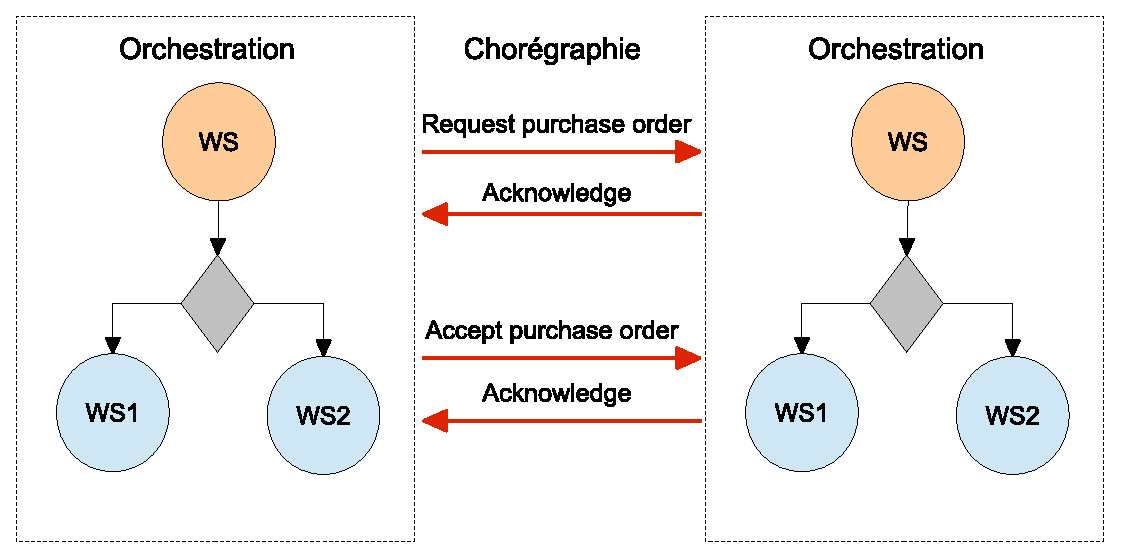
\includegraphics[width=1\textwidth]{figs/orchestration-vs-choregraphie.eps}
    \caption{Orchestration vs Chorégraphie selon Peltz
      \cite{peltz2003web}.}
    \label{fig:orchestration-vs-choregraphie}
\end{figure}       

      \subsubsection{Orchestration}
      \label{sec:orchestration-sec}
      Selon Sonia \emph{et al.} \cite{jamal2005environnement}:
      \emph{``L'orchestration des services Web permet de définir
        l'arranegement et l'enchaînement de ces services selon un
        canevas bien défini. Elle décrit la manière par laquelle les
        services peuvent interagir ensemble tout en incluant l'ordre
        d'exécution des différentes interactions''}.

      Barros \emph{et al.} \cite{barros2006standards} définissent
      l'orchestration comme un ensemble de processus exécutés dans un
      ordre prédéfini afin de répondre à un but
      \cite{lopez2008selection}. Ce type de composition se base sur un
      procédé métier exécutable permettant de décrire d'enchaînement
      et les interactions des différents services basiques collaborant
      dans une composition.
      
      L'orchestration offre \textbf{une vision centralisée} de
      contrôle, le procédé est toujours contrôlé par l'un des
      partenaires métiers. Ce dernier joue le rôle d'un chef
      d'orchestre qui se charge d'appeler les services de la
      composition suivant l'ordre d'exécution déjà défini par le
      processus métier. Le principe de l'orchestration est illustré
      par La figure \ref{fig:orchestration}.
      %TODO: citer qulques languages d'orchestration
      %TODO: les avantages et les inconvénients

      \subsubsection{Chorégraphie}
      \label{sec:choregraphie-sec}
      Selon Sonia \emph{et al.} \cite{jamal2005environnement} :
      \emph{`` La chorégraphie permet de tracer la séquence de
        messages échangés dans un contexte de composition de services
        Web. Elle est typiquement liée à la description de
        conversations existantes entre les services tout en impliquant
        plusieurs parties, incluant les clients, les fournisseurs et
        les partenaires''}.

      D'après Barros \emph{et al.} \cite{barros2006standards}, la
      chorégraphie permet de décrire la composition comme un moyen
      d'atteindre un but commun en utilisant un ensemble de services
      Web. La collaboration entre chaque service Web de la collection
      (faisant partie de la composition) est décrite par des flots de
      contrôle \cite{lopez2008selection}.

      La chorégraphie offre \textbf{une vision décentralisée} et
      \textbf{globale} du système et exprime une vue d'ensemble des
      services interagissant dans le cadre d'une composition de
      services. Selon Peltz \cite{peltz2003web}, la chorégraphie
      illustre les différants échanges de messages entre les
      participants. Le principe de la chorégraphie est illustré par la
      figure \ref{fig:choregraphie}.
      %TODO: citer qulques languages de chorégraphie.
      %TODO: les avantages et les inconvénients.

    \subsection{Stratégies de composition}

    \label{sec:types-de-composition}
    Un modèle de composition de service peut être relativement
    complexe. Il requiert la description et l'organisation de
    l'interaction entre les services et nécessite la gestion de
    plusieurs aspects comme les échanges de données entre les
    services, les pannes ou erreurs éventuelles, le contexte
    d'interaction, le degré d'automatisation des tâches, etc.
    
    Il existent une variété de spécifications, de langages et
    d'approches formelles développées par la littérature concernant la
    composition. Ces techniques sont également classés en fonction de
    différents dimensions, et selon les travaux effectués dans le
    champ des services web, les définitions des types de composition
    diffèrent d'une communauté de l'autre.

    Barros \emph{et al.} \cite{barros2006standards} classent la
    composition des services Web en trois catégories : la composition
    comportementale, l'orchestration et la chorégraphie, à l'instar de
    Barros \emph{et al.}, Peltz \cite{peltz2003web} considère les
    procédés de coordination \ref{sec:proc-de-coord} et distingue
    seulement les deux dernières \textit{(orchestration,
      chorégraphie)}.
  
    %% commment classifies la compositions ?
    %% \cite{fluegge2006challenges} Static vs dynamique.

    %% Les Procédés de coordination comme une vision (point de vue)
    %% d'une composition des services Web.

    % TODO: vertical vs horiontal composition
    Medjahed.\cite{medjahed2004thesis} de ça part définit trois types
    de composition selon...
    % the composition mode refers to the way participants are
    % combined. We define three composition types: horizontal, vertical,
    % and hybrid. Horizontal compo- sition refers to a “supply
    % chain”-like combination of Web services.  Vertical composition
    % refers to the “outsourcing” of a Web service by a sub-request or
    % another Web service. Horizontal composition implies the combina-
    % tion of several Web services. It is hence used with one-to-many
    % cardinality. Vertical composition refers to the outsourcing of one
    % Web service. It is hence combined with one-to-one
    % cardinality. Hybrid composition refers to the most general mode.
    % It may be used with both horizontal and vertical compositions

    % TODO: les procédés de coordination selon [fluegge2006challenges]
    % TODO

    % Microsoft Biztalk et Bea WebLogic sont deux exemples de moteurs
    % de composition statiques de services Web. Pour la composition
    % dynamique, nous trouvons les plate-formes e-flow de HP et Sword
    % de Stanford.

    % Dans le cadre d'une composition statique de services, si les
    % fournisseurs proposent d'autres services ou changent les anciens
    % services, des incohérences peuvent être causées. Ceci qui
    % demande un changement de l'architecture du logiciel, voire de la
    % définition de l'application et crée l'obligation de faire une
    % nouvelle conception de l'application. C'est pourquoi, la
    % composition statique des services web est considérée rigide et
    % trop ee restrictive [86 S. Sanlaville, Environnement de proc ́d ́
    % extensible pour l'orchestration : Application aux services e e
    % web, Ph.D. Thesis, 2005 ]
    % \cite{driss2011approche}

      % \subsubsection{Composition horizontale/verticale}
      % \label{sec:comp-horiz}
      % D'autres travaux s'intressent à ... comme
      % \cite{medjahed2004thesis}.

    
      \subsubsection{Composition statique/dynamique}
      \label{sec:comp-stat}
      Selon la disponibilité des services composites, La composition
      des services Web peut être soit une composition statique soit
      une composition dynamique

      \SpecialItem
      \begin{description}
      \item[Composition statique] :

        % est appelé aussi composition off-line, précompil ou encore
        % proactive. C'est une composition qui utilise des services
        % basiques qui sont au préalablement d éfinis d'une façon figée
        % et qui ne peuvent pas changer en fonction du contexte du
        % client. Ce type de composition engendre des applications peu
        % flexibles, parfois inappropriées avec les exigences des
        % clients.  \cite{driss2011approche}

        % Permet de créer de nouveaux services composites à partir des
        % services déjà existants dans des environnements « stables » où
        % les services Web participants sont toujours disponibles et où
        % le comportement du service composite est le même pour tous les
        % clients. La composition des services web prend place durant la
        % période de conception. Les composants sont choisis, reliés
        % entre eux et enfin compilés et déployés. Le service composite
        % ainsi obtenu fonctionnera bien tant que son environnement et
        % les services qui le composent ne changent pas ou ne changent
        % que rarement. Microsoft BizTalk est un exemple de moteurs de
        % composition statique. Ce type de composition est utile pour
        % mettre en place des services composites qui implémente des
        % services métiers connus et très souvent sollicités dans un
        % domaine donné (donc communs à plusieurs utilisateurs), par
        % exemple : achat d’un véhicule, planification d’un voyage...etc
        % . C'est d'ailleurs la raison pour laquelle ces approches se
        % limitent à un schéma d'orchestration (ou de chorégraphie)
        % prédéfini pour décrire les besoins préalablement connus de
        % l'utilisateur. \cite{ch3}

      \item[Composition dynamique] :

        % appelée aussi composition on-line, postcompilée ou encore
        % réactive. Elle se réfère à la sélection des services basiques
        % àla volée. Autrement dit, la sélection des services basiques
        % ne peut pas être pr définie à l'avance mais elle sera faite au
        % moment de l'exécution en fonction des contraintes imposées par
        % le client. Ceci permet d' élaborer différents scénarii de
        % composition qui offrent les mêmes fonctionnalités et qui
        % tiennent compte de la dynamique de la situation du client.
        % \cite{driss2011approche}

        % Dans ce type, les services Web à composer sont déterminés lors
        % de l’exécution de la requête d’un client. Ils peuvent être
        % déterminés selon les contraintes de chaque client, la
        % disponibilité des services Web, ...etc. La composition
        % dynamique apparaît la plus intéressante d’une part,elle promet
        % d'être capable de faire face à un environnement très dynamique
        % dans lequel des services apparaissent et disparaissent
        % rapidement. La composition des services web implique : - La
        % découverte des « bons » services à composer selon les besoins
        % et la disponibilité des services.  - La dynamicité et la
        % flexibilité dans la composition de services Web. \cite{ch3}
      \end{description}

      \subsubsection{Composition manuel/automatique}
      \label{sec:comp-manu}
      Classification basée sur le degré d'automatisation.

      \SpecialItem
      \begin{description}
      \item[Composition manuel] :
      \item[Composition semi-automatique] :
      \item[Composition automatique] :

        % La composition automatique (dynamique par le terme de
        % \cite{fluegge2006challenges} permet un développement plus
        % rapide des applications à base de services. Elle consiste à
        % préciser la requête d'un utilisateur sous forme d'objectifs à
        % satisfaire. Un moteur de composition \textit{``intelligent''}
        % choisit la comabinaison de services répondant à l'objectif
        % décrit. Il génère la composition de service adéquate de
        % manière transparente à l'utilisateur. Ce principe a interpellé
        % plusieurs communautés de recherche travaillant dans le domaine
        % de l'Intelligence Artificielle.  \cite{elie2010}
      \end{description}

      % TODO introduire la classification \cite{fluegge2006challenges}
      % TODO introduire les procédés de coordination par
      % \cite{peltz2003web}
      % \ref{sec:lang-de-comp}...
      % Dans la suite, les types de composition des
      % services Web désigne types classés par\cite{fluegge2006challenges}.        
  \section{Langages pour la composition}
  \label{sec:lang-de-comp}
  % TODO: an introduction to the section
  % TODO: re-draw figs an unify them
  % Afin de supporter la composition de services, plusieurs langages de
  % composition de services ont été proposés comme ...  Dan cette
  % section on va détailler trois langages ... \cite{lopez2008selection}
  % % TODO change the font of commands in BPEL et al....

  %   \subsection{BPEL}
  %   \label{sec:bpel}

  %   \acrshort{bpel} est une spécification du consortium OASIS
  %   \footnote{\url{https://www.oasis-open.org}}issue de la fusion des
  %   spécifications \acrshort{xlang} Microsoft
  %   \footnote{\url{http://www.microsoft.com}}et \acrshort{wsfl} d'IBM
  %   \footnote{\url{http://www.ibm.com}}, il hérite les
  %   caractéristiques d'un langage structuré en blocs de
  %   \textsc{XLANG}, ainsi que les caractéristiques d'un graphe direct
  %   de WSFL \cite{driss2011approche}.

  %   \begin{figure}[h]
    \centering
    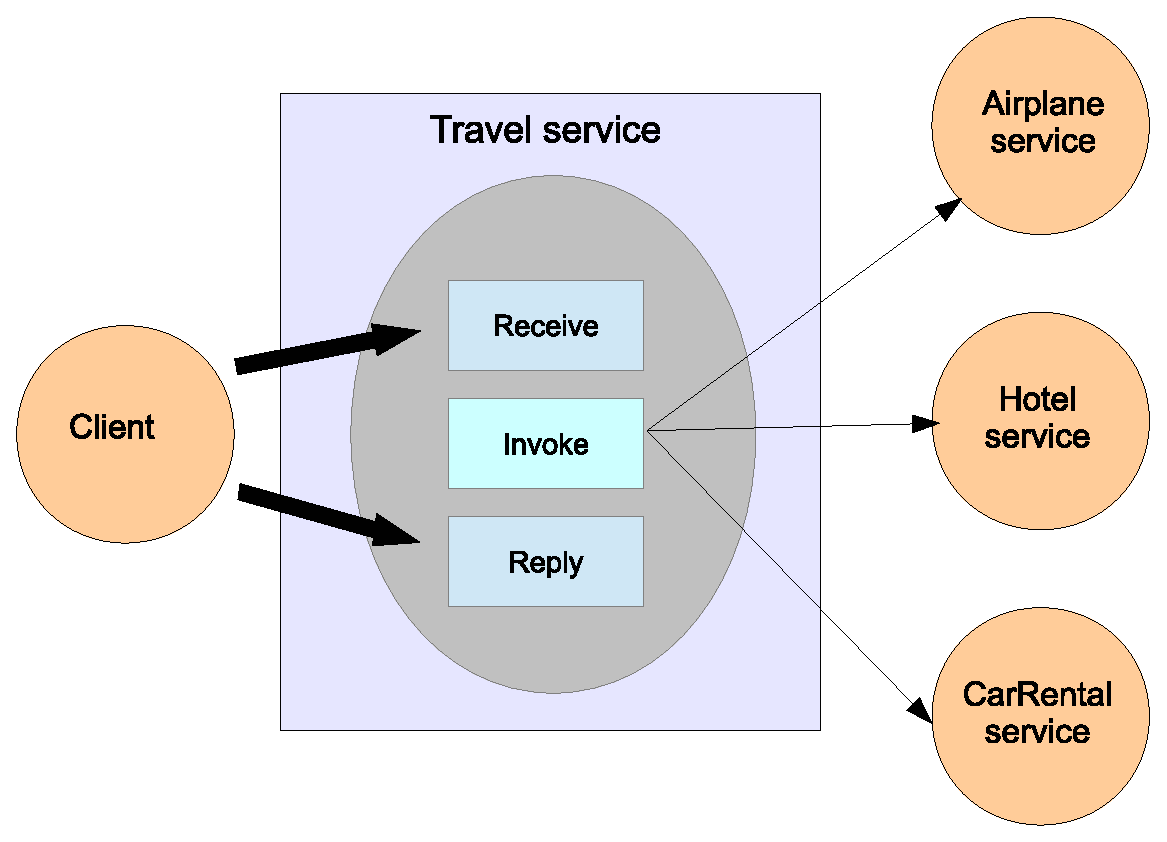
\includegraphics[width=0.8\textwidth]{figs/bpel-travel-example-shema.eps}
    % TODO translate the figure
    % TODO reference the fig
    \caption{Une vue interne de service de voyage \textsc{bpel}.}
    \label{fig:3w_to_sws}
\end{figure}
%%% Local Variables: 
%%% mode: latex
%%% TeX-master: "3w_to_sws"
%%% End: 


  %   \textsc{BPEL} \textit{(appelé aussi \acrshort{bpel4ws} ou
  %     \acrshort{ws-bpel})} est le langage d'\textbf{orchestration}
  %   le plus utilisé dans l'industrie permettant la coordination des
  %   interactions entre l'instance du service composite et ses
  %   partenaires sous forme d'un schéma \acrshort{xml} \textit{(le
  %     script d'orchestration)}, il définit le processus,
  %   l'enchaînement et l'ordonnancement des actions qui seront
  %   exécutées par le moteur d'orchestration, agissant comme une
  %   machine virtuelle capable d'exécuter \textbf{le procédé métier}
  %   intéreptable de \textbf{coordination} \cite{chollet2009orchestration}.

  %   \textsc{BPEL} repose sur un modèle constitué d'activités de
  %   coordination qui peuvent être de deux types, les activités de base
  %   ou élémentaires comme l'invocation (invoke) d'un service,
  %   l'attente d'une réponse et la génération d'une réponse (reply), et
  %   les activités composites permettant du contrôle du flot de données
  %   comme les séquences (sequence), les exécutions en parallèle (flow)
  %   et les branchements (switch, if). La figure
  %   \ref{fig:bpel_travel_example_document} représente une opération de
  %   type ``séquence'' illustrée dans le shémas
  %   \ref{fig:bpel-travel-example-schema}.

  %   \begin{figure}[h]
    \centering
    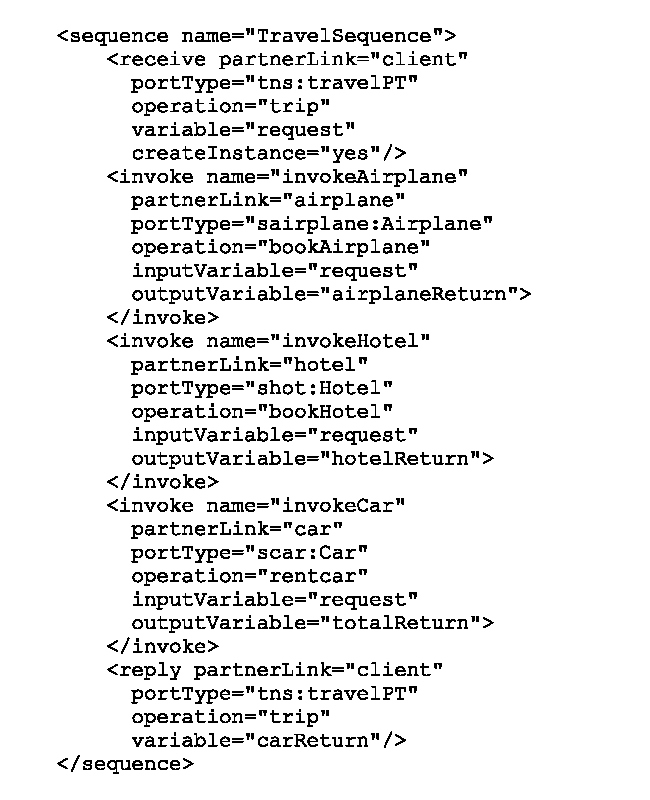
\includegraphics[width=0.8\textwidth]{figs/bpel_travel_example_document.eps}
    % TODO translate the figure
    % TODO reference the fig
    \caption{Le procédé d'orchestration de service de voyage \textsc{bpel}.}
    \label{fig:bpel_travel_example_document}
\end{figure}



  %   %% procédé abstraite vs exécutable Selon \cite{chollet2009orchestration}
  %   % WS-BPEL est un langage de procédés basé sur la technologie XML,
  %   % tout comme les autres standards des services Web. WS-BPEL permet
  %   % de construire des procédés interprétables et exécutables par un
  %   % moteur d'orchestration.

  %   % Les procédés peuvent être modélisés de deux manières :
  %   % – abstraite : seuls les échanges de messages entre les
  %   % différents participants sont spécifiés. Mais le comportement
  %   % interne de ces participants n'est pas explicité.
  %   % – exécutable : les activités du procédé sont ordonnées; les
  %   % partenaires impliqués sont identifiés ainsi que les messages
  %   % qui sont échangés. A ceci s'ajoute le traitement des fautes
  %   % et des exceptions pour les cas d'erreurs.

  %   % inclut la sémantique ?
  %   % TODO: avantages et inconvénient

  %   \subsection{WS-CDL}
  %   \label{WS-CDL}
  %   % make a reference to [TODO: Kavantzas et al., 2005] selon
  %   % elie2010
  %   \acrshort{ws-cdl} est un langage de composition de services de
  %   type \textbf{chorégraphie} qui permet de décrire une vision
  %   \textbf{globale} des collaborations entre les services Web
  %   \cite{elie2010}, à l'instar des standards de services Web,
  %   \textsc{WS-CDL} est basé sur \textsc{XML}, il complète la
  %   description \acrshort{wsdl} des services Web afin de décrire les
  %   interactions entre les participants (les services Web) de la
  %   composition.

  %   \textsc{WS-CDL} reprend et développe la spécification
  %   \acrshort{wsci} décrivant les séquences ordonnées de messages
  %   impliquant plusieurs entités (services Web) engagés dans une
  %   composition visant à accomplir un objectif commun.

  %   \textsc{WS-CDL} consiste à définir un fichier XML décrivant une
  %   chorégraphie, il permet de \cite{elie2010}:
  %   \begin{itemize} % WSDL-S elements and attributs
  %   \item désigner les variables et les types de données échangées.
  %   \item décrire les  activités impliquées.
  %   \item décrire les structures illustrant les interactions entre
  %     les activités.
  %   \end{itemize}

    %       En résumé WS-CDL permet de décrire les règles selon
    %       lesquelles une collaboration doit avoir lieu. Il fournit une
    %       structuration globale de l'interaction en fonction de
    %       laquelle chaque participant décrit son processus métier et
    %       par suite ses services.
    %  \cite{elie2010}

    %  WS-CDL (Web Service Choreography Description Language) est un
    %  langage issu des efforts de standardisation
    %  du groupe de travail du W3C portant sur la chorégraphie de
    %  services Web (Web Services Choreography Working
    %  Group52). L'objectif de ce langage est de décrire les relations
    %  entre les services Web lors d'une composition de type
    %  chorégraphie.

    %  WS-CDL est un langage de composition de services de type
    %  chorégraphie définissant des contrats multi-parties. L’avantage
    %  de ce langage est que la description des interactions (l’élément
    %  Choreography du Package) est réutilisable. Ceci permet de
    %  diminuer la charge de travail des concepteurs. L’inconvénient de
    %  WS-CDL est que même si l’élément Choreography est réutilisable,
    %  sa description reste lourde. Un service doit posséder autant de
    %  Package que de participations à des compositions. De plus, WS-CDL
    %  n’inclut pas pour le moment de sémantique. Des travaux, tels que
    %  [Kang et al., 2007a] et [Kang et al., 2007b], proposent d’étendre
    %  WS-CDL afin d’y intégrer de nouveaux concepts (tels que la
    %  gestion des erreurs et des exceptions ou la mise en œuvre d’un
    %  minuteur d’exécution de la composition).

     % \cite{lopez2008selection}

    % TODO: shémas exemple d'un document WS-CDL.
    % inclut la sémantique ?
    % TODO: avantages et inconvénients.

    % \subsection{OWL-S}
    % \label{sec:owl-s}
    % \cite{mcilraith2003bringing}
    % \begin{figure}[h]
    \centering
    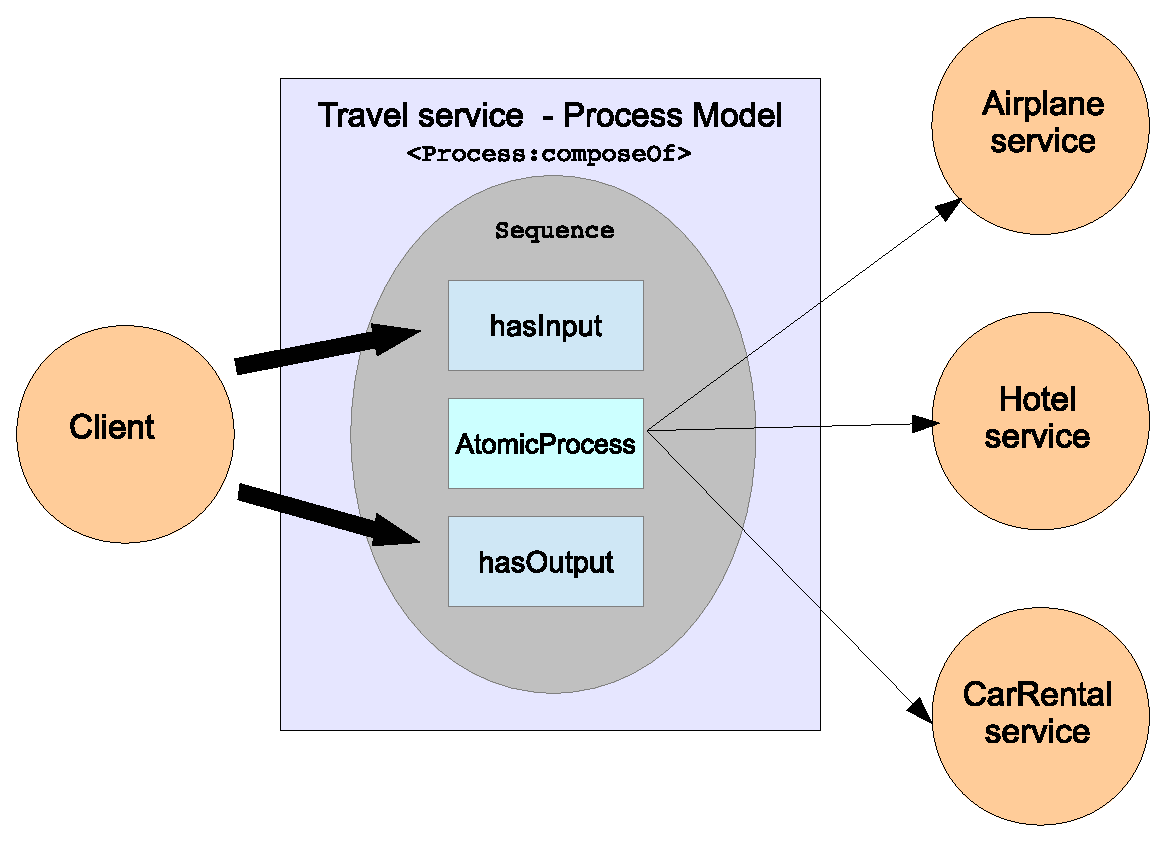
\includegraphics[width=0.8\textwidth]{figs/owls_travel_example_schema.eps}
    % TODO translate the figure
    % TODO reference the fig
    \caption{Une vue interne d'un service de
      voyage composite\textsc{owls}.}
    \label{fig:owls-travel-example-schema}
\end{figure}
%%% Local Variables: 
%%% mode: latex
%%% TeX-master: "3w_to_sws"
%%% End: 

    % \begin{figure}[h]
    \centering
    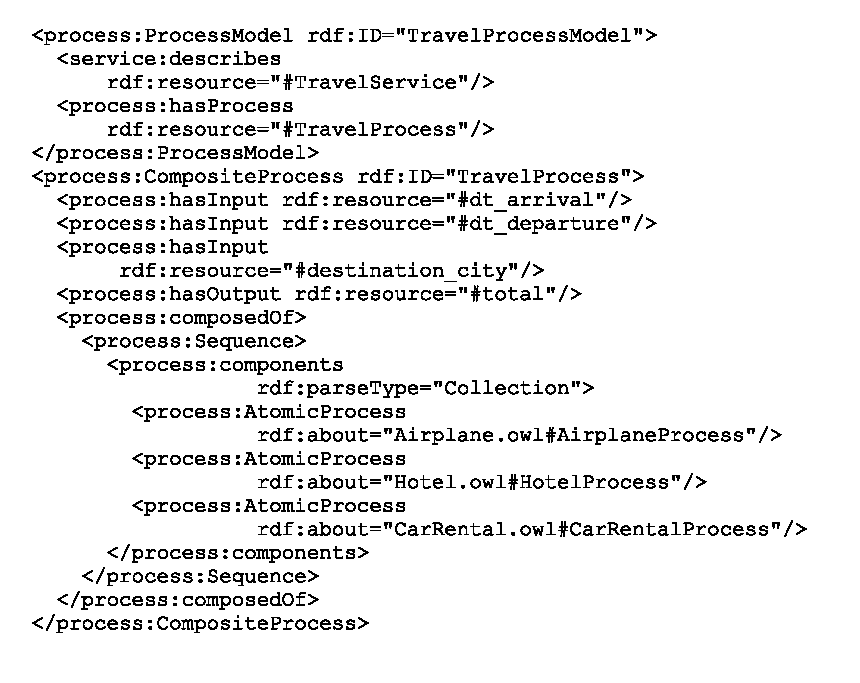
\includegraphics[width=1.1\textwidth]{figs/owls_travel_example_document.eps}
    % TODO translate the figure
    % TODO reference the fig
    \caption{Document OWLS de processus composite du service de voyage \textsc{bpel}.}
    \label{fig:owls_travel_example_document}
\end{figure}

    % % see the BPEL reference for a complete schema and example

  \section{Composition dynamique des services web}
  \label{sec:comp-dynam}


  % les motivation de la composition dynamiques [\cite{bartalos2011effective}]
  % The motivation for service orchestration as just mentioned is more about solving
  % technical problems related to the software integration. Unfortunately, the overall
  % principles of SOA are not fully adapted and used in practice. During the last years
  % there has been a vision that Web services could be automatically arranged to
  % supply a complex functionality. A lot of research effort has been made to develop
  % approaches able to find and arrange relevant services in a meaningful, optimal
  % manner to satisfy the goal defined by the requestor. This idea moves toward the
  % exploitation of single services. However, the complexity of single services is not
  % limited, it is not effective, or it is even impossible to develop services satisfying all
  % possible (expected) requests. Thus, other methods must be investigated to be able
  % to supply variable functionality. A more feasible approach is to arrange several
  % simpler services on the fly (dynamically) based on the given request. This is called
  % also explorative service composition (Yang and Papazoglou, 2004).



  % There are several principal differences between the situation when the Web
  % services are used to realize some activities prescribed by a business process and the
  % situation when they are automatically arranged on the fly to supply the need of the
  % requestor. In the situation when the arrangement of services, i.e. orchestration,
  % is done based on the given business process, it is made manually by a software
  % developer. The resulting arrangement is realizing a defined task for a long period
  % of time, for multiple users. In the second situation, the arrangement is done
  % automatically, based on the descriptions of the available services and the given
  % user goal. In this case we will call it service composition. This approach suits well
  % also in the case when the user goal is varying and the situation requires flexible
  % arrangement of services.

  % Service composition is also possible in the case when the number of potential
  % services is very high. The manual composition is not effective, or is even impossible
  % in this case. On the other side, the service orchestration does not require additional
  % description of services, since the developers can use the documentation of the used
  % services. Service composition relies on additional metadata about services, to make
  % them distinguishable and understand what functionality they realize. These must
  % be provided in a standardly defined form.

  % The automatic dynamic Web service composition introduces new possibilities
  % in the area of Web services (Dustdar and Papazoglou, 2008; Dustdar and Schreiner,
  % 2005). Its aim is not to solve existing problems with the manual composition, or
  % automate this process. The manual composition still has its place in the software
  % development process of on-demand software solutions based on the given require-
  % ments. The automatic dynamic composition provides the opportunity to exploit
  % the available services to supply a wide range of varying user goals.

  La classification est d'aprés \cite{baryannis2010}.

    \subsection{Les approches basées sur les workflow}
    \label{sec:les-approches-basees}

    \subsection{Les approches guidées par les modèles}
    \label{sec:les-appr-guid}

    \subsection{Les apprcohes mathématiques}
    \label{sec:les-apprc-math}
   
    \subsection{Techniques de planification}    
    \label{sec:techn-de-plan}
    Selon \\cite{baryannis2010} et\cite{bartalos2011effective}.


  \section{Conclusion}
  \label{sec:conclusion}
    % conclusion
  Introduire la composition dynamique basé sur le modèle graphe qui se
  sera détaillé dans le prochain chapitre.
  % TODO rapeller du problème initiale en contexte de ce chapitre en une
  % page
 

%%% Local Variables: 
%%% mode: latex
%%% TeX-master: "../main"
%%% End:
%  LocalWords:  web Barros Peltz différants BPEL bpel xlang Microsoft
%  LocalWords:  wsfl d'IBM ws ws-bpel xml WS-CDL ws-cdl wsdl wsci
%  LocalWords:  OWL-S
